\documentclass{article}

% if you need to pass options to natbib, use, e.g.:
%     \PassOptionsToPackage{numbers, compress}{natbib}
% before loading neurips_2020

% ready for submission
% \usepackage{neurips_2020}

% to compile a preprint version, e.g., for submission to arXiv, add add the
% [preprint] option:
%     \usepackage[preprint]{neurips_2020}

% to compile a camera-ready version, add the [final] option, e.g.:
%     \usepackage[final]{neurips_2020}

% to avoid loading the natbib package, add option nonatbib:
\PassOptionsToPackage{numbers, compress}{natbib}
\usepackage{neurips_2020}
\usepackage[cache=false]{minted}
%\usepackage[utf8]{inputenc} % allow utf-8 input
\usepackage[T1]{fontenc}    % use 8-bit T1 fonts
\usepackage{hyperref}       % hyperlinks
\usepackage{url}            % simple URL typesetting
\usepackage{booktabs}       % professional-quality tables
\usepackage{amsfonts}       % blackboard math symbols
\usepackage{nicefrac}       % compact symbols for 1/2, etc.
\usepackage{microtype}      % microtypography
\usepackage{amsmath}
\usepackage{wrapfig}
\usepackage{clrscode3e}

%\usepackage{newunicodechar}
%\usepackage{fontspec}
%\newfontface\mathsymbolfont{Latin Modern Math}
%\newunicodechar{ϕ}{{\mathsymbolfont\mitphi}}

\newenvironment{tab}[2][\linewidth]
{\begin{tabular*}{#1}[t]{@{\extracolsep{\fill}}>{\hspace{4pt}}#2}}%
{\end{tabular*}}

\usepackage{trimspaces}
\newcommand*{\trim}[1]{%
  \trim@spaces@noexp{#1}%
}
\usepackage{tikz}
\usetikzlibrary{decorations.pathreplacing,shapes,arrows,positioning,calc}

\tikzset{
  cfedge/.style={
    font=\itshape,
    draw=black,
    ->,
    >=stealth'
  },
  process/.style={
    draw,
    fill=orange!50,
    rectangle,
    minimum height=1.5em,
    minimum width=4em,
    align=center,
    font=\small,
  }
}

\newcommand{\todo}[1]{{\color{red} TODO: #1}}
\newcommand{\wmnote}[1]{{\color{blue} Billy: #1}}
\newcommand{\vcnote}[1]{{\color{yellow} Valentin: #1}}
\newcommand{\define}[1]{\textbf{\emph{#1}}}

\title{Instead of Rewriting Foreign Code for Machine Learning, Automatically Synthesize Fast Gradients}

\author{%
  David S.~Hippocampus\thanks{Use footnote for providing further information
    about author (webpage, alternative address)---\emph{not} for acknowledging
    funding agencies.} \\
  Department of Computer Science\\
  Cranberry-Lemon University\\
  Pittsburgh, PA 15213 \\
  \texttt{hippo@cs.cranberry-lemon.edu} \\
  % examples of more authors
  % \And
  % Coauthor \\
  % Affiliation \\
  % Address \\
  % \texttt{email} \\
}

\begin{document}
\bibliographystyle{plainnat}

\maketitle


\begin{abstract}
Applying differential programming techniques and machine learning algorithms to foreign programs requires developers to either rewrite their code in a machine learning framework, or otherwise provide derivatives of the foreign code.
This paper presents Enzyme, a high-performance automatic differentiation (AD) compiler plugin for the LLVM compiler framework capable of synthesizing gradients of statically analyzable programs expressed in the LLVM intermediate representation (IR). Specifically, Enzyme can synthesize gradients for programs written in any language whose compiler targets LLVM IR including C, C++, Fortran, Julia, Rust, Swift, MLIR, etc., thereby providing native AD capabilities in these languages. Unlike traditional source-to-source and operator-overloading tools, Enzyme performs AD on optimized IR. On a machine-learning focused benchmark suite including Microsoft's ADBench, AD on optimized IR achieves a geometric mean speedup of 2.851x\todo{put real number} over AD on IR before optimization. Packaging Enzyme for PyTorch and Tensorflow provides convenient access to gradients of foreign code with state-of-the art performance, enabling foreign code to be directly incorporated into existing machine learning workflows. 
\end{abstract}

\section{Introduction}
\label{sec:intro}

Machine learning frameworks such as PyTorch~\cite{paszke2017automatic} and Tensorflow~\cite{abadi2016tensorflow} have become widespread as the primary workhorses of the modern machine learning community. In order to compute the necessary gradients for algorithms such as backpropagation~\cite{hecht1992theory}, bayesian inference, and uncertainty quantification~\cite{Wang2018-yr}, however, programmers are required to rewrite all of their code to be in said framework. This rewriting is especially problematic for applying machine learning to new domains as existing tools like physics simulators~\cite{feng2016fastpm, broughton2020tensorflow, NIPS2018_7948, degrave2019differentiable, hu2019difftaichi}, game engines, climate models~\cite{Stevens2020-ir}, and medical models~\cite{alquraishi2019end} that are not written in the domain specific languages of machine learning frameworks. High performance automatic differentiation is also necessary for probabilistic programming frameworks~\cite{cusumano2019gen}.

This rewriting has been identified as the quintessential challenge of applying machine learning to scientific computing~\cite{Baker2019-ty}. As stated in \citet{10.15200/winn.156631.13064} ``This is [the key challenge of scientific ML] because, if there is just one part of your loss function that isn't AD-compatible, then the whole network won't train.''

To remedy this issue, the trend has been to create new domain-specific languages (DSL) \todo{hu2019difftaichi, more citations} that make the rewriting process easier or to integrate differentiation as a first-class construct in programming languages to enable differential programming ($\delta P$)~\cite{maclaurin2015autograd,jax2018github,SwiftAutodiff,zygoteMlsys}. This results in efficient gradients, but still requires rewriting in either the DSL or the differential programming language. 


To use existing code that is foreign to the Machine Learning framework developers can use reverse-mode AD frameworks that operate on the foreign language. 

\todo{You don't have to write complicated losses in tensorflow math world;}

In languages without an existing first-class AD framework, there have been two approaches to computing gradients.

\define{Operator-overloading} approaches take advantage existing language functionality compute derivatives of functions alongside the original code. Examples of this include Adept~\cite{adept} and ADOL-C~\cite{griewank1996algorithm}, C++ libraries that provide differentiable versions of primitive types or JaX~\cite{jax2018github} and AutoGrad~\cite{maclaurin2015autograd} are Python libraries that provides derivatives NumPy-style functions. These approaches, however, require rewriting your source code to use the differentiable types/operations in place of standard language utilities and thus also cannot differentiate many libraries, nor any code in other languages.
% , and can often be slow as they must store what operations are taking place in order to later differentiate.

\define{Source-rewriting}~\cite{10.5555/1455489} approaches analyze the source code of programs and emit new source code that computes the derivative of a function. Examples include Tapenade~\cite{TapenadeRef13}, a framework which computes forward and backwards mode derivatives for C and Fortran programs; ADIC~\cite{narayanan2010adic2} another source-rewriter for C and C++; and Zygote~\cite{zygoteArxiv,zygoteDP,zygoteMlsys}, a framework that dynamically generate derivative functions in Julia. Such tools can be more efficient than operator-overloading approaches as they can statically analyze the computation. They also tend to only work with programs in a specific language, sometimes even only a subset of programs in that language. They also require all of the source to be differentiated to be available to the tool. This makes them difficult to use with header-only libraries and impossible to use with precompiled libraries.

Moreover, as more codebases use libraries from other languages, it is necessary to compute gradients of functions from many languages in the same framework. Tapenade is able to do this between C and Fortran~\cite{pascual2016mixed}.\todo{discuss other cross language AD}

\begin{figure*}
    \centering
\begin{minted}[fontsize=\small]{c}
double mag(const double* x);//Compute magnitude in O(N)
void norm(double* out, double* in) {
    // double res = mag(in); code motion optimization can move outside the loop
    for(int i=0; i<N; i++) { out[i] = in[i]/mag(in); }
}
\end{minted}
\begin{tabular}{c|c}
\begin{minipage}[T]{0.49\linewidth}
\begin{minted}[fontsize=\small]{c}
// LICM, then AD, O(N)
void norm(double* out, double* dout,
         double* in, double* din) {
  double res = mag(in);
  for(int i=0; i<N; i++) {
    out[i] = in[i]/res;
  }
  double dres = 0;
  for(int i=0; i<N; i++) {
    dres += -in[i]*in[i]/mag * dout[i];
    din[i] += dout[i]/mag;
  }
  dmag(in, din, dres);
}
\end{minted}
\end{minipage}& \begin{minipage}[T]{0.49\linewidth}
\begin{minted}[fontsize=\small]{c}
// AD, then LICM O(N^2)
void norm(double* out, double* dout,
          double* in, double* din) {
  double res = mag(in, n);
  for(int i=0; i<n; i++) {
    out[i] = in[i]/res;
  }
  for(int i=0; i<n; i++) {
    double dres = -in[i]*in[i]/mag \
                        * dout[i];
    din[i] += dout[i]/mag;
    dmag(in, din, n, dres);
  }
}
\end{minted}
\end{minipage}
\end{tabular}
    \caption{In the second program, mag is still able to be moved outside as it is the same every iteration, however, \texttt{dmag} cannot be moved outside the loop as it reads/writes to the same memory.
}
    \label{fig:licm}
\end{figure*}

Both operator-overloading and source-rewriting AD systems differentiate programs before optimization. Optimizations can  significantly reduce the work in a program by deleting and simplifying instructions. Performing AD on an unoptimized program requires will create longer and more complex backwards passes, which may not be optimizable. Consider the program at the top of Figure~\ref{fig:licm} that normalizes a vector. A smart compiler will move the $O(N)$ call to \texttt{mag} outside the loop, changing the runtime of the code from $O(N^2)$ to $O(N)$ by an optimization known as loop-invariant-code-motion (LICM)~\cite[Sec.~13.2]{Muchnick97}. Running LICM then AD results in the $O(N)$ code on the left with both \texttt{mag} and its adjoint \texttt{dmag} are outside the loop. However, if AD is run before LICM, the forward pass will have \texttt{mag} outside the loop, however AD will call the adjoint \texttt{dmag} inside the loop. LICM cannot move \texttt{dmag} outside the loop as it uses a value computed inside the loop.

Traditional AD systems have not been able to operate on optimized IR as it either requires re-implementing all of the compiler optimizations or working at a low level after which optimization has already been performed. It has conventionally believed to be hard to produce efficient gradients for low-level code as it lacks high-level information many AD tools rely upon. As described in \citet{zygoteArxiv}, ```AD is more effective in high-level compiled languages (e.g. Julia, Swift, Rust, Nim) than traditional ones such as C/C++, Fortran and LLVM IR [...].''' The LLVM~\cite{LLVM} compiler toolchain defines a low level intermediate representation (IR) and provides a set of optimizations used by many compiler toolchains.

This paper presents Enzyme, an efficient cross-platform compiler plugin for automatic differentiation that operates on LLVM IR~\cite{LLVM} and makes the following contributions:
\begin{itemize}

\item Enzyme, a compiler plugin for LLVM that can synthesize high-performing gradients of statically analyzable LLVM IR, including IR generated by compiler frontends for C, C++, Fortran, Nim, Rust, Swift, and others.

\item PyTorch-Enzyme, a foreign-function interface for the PyTorch machine learning framework that allows programmers to use code written in LLVM-compiled languages in their machine-learning workflows, as well as a similar foreign-function interface for TensorFlow.

\item Enzyme.jl, a package that uses Enzyme to synthesize high-performing gradients of Julia code, which demonstrates that gradients of code written in a dynamic high-level language can be generated statically and perform well with only low-level information.

\item A study demonstrating that running AD after optimization results in significant performance gains on a standard machine learning benchmark suite~\cite{adBench} and achieve state-of-the-art performance with other AD systems.

\todo{thoughts of multisource or clang native AD}
\end{itemize}

\paragraph{Related work}

Clad is a plugin to the Clang compiler that implements forward automatic differentiation on a subset of C/C++ with reverse mode in development~\cite{Vassilev_Clad}. \citet{chen2018neural} present an end-to-end differentiable model for protein structure prediction. 
DiffTaichi~\cite{hu2019difftaichi} implements a differential DSL for physics and robotics simulation. \citet{NIPS2018_7948} also provides a differential physics framework. Halide is a differentiable DSL for image processing~\cite{Li:2018:DPI}. Swift implements first class automatic differntiation~\cite{SwiftAutodiff}. A compiler plugin to provide differentiable programming in Haskell~\cite{Elliott2018-gr}.


\section{Design}
\label{sec:design}

Enzyme is composed of three stages: \define{type analysis} determines the underlying types of values, \define{activity analysis} determines what instructions and values can impact the gradient calculation, and \define{synthesis} creates the necessary functions to compute the gradient. A core design goal of Enzyme is to operate upon optimized IR. As seen in Figure \ref{fig:licm} this can result in significant benefits such as more simpler and more optimized gradients, though requires working on a low-level representation.

Gradients synthesized by Enzyme contain two parts: a \define{forward pass} that mirrors the original code and a \define{reverse pass} that computes the gradient by inverting the instructions in the forward pass. Inverted instructions in the reverse pass are known as \define{adjoint}s. For all differentiable instructions in LLVM, Enzyme defines an adjoint to describe how gradients propagate through the instructions.

\subsection{Type Analysis}
One challenge of performing AD on LLVM IR (and even C/C++) is that LLVM types do not necessarily represent the type of the underlying data. For example, the \texttt{memcpy} function copies data between generic pointers without types (\texttt{void*}). Creating a correct gradient for \texttt{memcpy}, however, requires knowing the type of the memory being copied. As shown in Figure \ref{fig:memcpy}, copying 8 bytes of double data requires performing one double (8-byte) addition in the reverse pass, whereas copying 8 bytes of float data requires two float (4-byte) additions. As these two operations are incompatible with each other (resulting in an incorrect gradient), Enzyme must be able to determine the type of the data being copied.

Enzyme does so by creating a new interprocedural type analysis. Every value in a function is given a \define{type tree} that describes the known type at any given byte offset in the value. If the type at a particular offset is a pointer type, we have a new type tree that represents the types inside that offset. As an example the type tree \verb|{[]:Pointer, [0]:Double, [8]:Integer}| represents a pointer to a struct that contains first a double at byte 0, then an integer at byte 8.

Type analysis initializes the type trees of all values to empty and uses type based alias analysis (TBAA) metadata to initialize the type trees of loads, stores, and \texttt{memcpy} operations.
TBAA allows us to make assumptions about the underlying type because of strict aliasing~\cite{10.1145/277650.277670, langref_2020}. For every kind of instruction, Enzyme implements a type propagation rule that specifies how types flow through the instruction. As an example, if the result of a load is known to be type \texttt{T}, then the pointer loaded must be a pointer to \texttt{T} at offset 0. Type analysis then runs all of the type propagation rules until a fixed point is reached.
\todo{connection to abstract interpretation}
\begin{figure*}
    \centering
\begin{minted}[fontsize=\small]{c}
void f(void* dst, void* src) { memcpy(dst, src, 8); }
\end{minted}
\begin{tabular}{c|c}
\begin{minipage}[T]{0.49\linewidth}
\begin{minted}[fontsize=\small]{c}
// Gradient memcpy for double inputs
void grad_f(double* dst, double* ddst,
            double* src, double* dsrc) {
  // Forward pass
  memcpy(dst, src, 8);
  // Reverse pass
  dsrc[0] += ddst[0];
  ddst[0] = 0;
  
  
}
\end{minted}
\end{minipage}&
\begin{minipage}[T]{0.49\linewidth}
\begin{minted}[fontsize=\small]{c}
// Gradient memcpy for float inputs
void grad_f(float* dst, float* ddst,
            float* src, float* dsrc) {
  // Forward pass
  memcpy(dst, src, 8);
  // Reverse pass
  dsrc[0] += ddst[0];
  ddst[0] = 0;
  dsrc[1] += ddst[1];
  ddst[1] = 0;
}
\end{minted}
\end{minipage}
\end{tabular}
\caption{{\textbf{\textit{Top:}}} Call to \texttt{memcpy} for an unknown 8-byte object. {\textbf{\textit{Left:}}} Gradient for a \texttt{memcpy} of 8bytes of double data. {\textbf{\textit{Right:}}} Gradient for a \texttt{memcpy} of 8bytes of float data. }
\label{fig:memcpy}
\end{figure*}

\subsection{Activity Analysis}
Activity analysis determines what instructions could impact the gradient computation and is common in automatic differentiation systems to avoid performing unnecessary adjoints~\cite{shin2007comparison}. Enzyme uses it to avoid taking gradients of instructions for which that would be ill defined (e.g. the \texttt{cpuid} instruction). An instruction is active iff it can propagate a differential value to its return or another memory location. For example a function that counts the length of a an active input array would not be active. In our implementation of activity analysis, we leverage LLVM's alias analysis~\cite[Ch.~12]{AhoLaSe06} and type analysis to help prove that instructions are inactive. As an example, any read-only function that returns an integer must be inactive since it cannot propagate adjoints through the return or any memory location.
\todo{think about expanding this rule}

\begin{figure}
\centering
\begin{tabular}{c|c}
\begin{minipage}[T]{0.42\linewidth}
\begin{minted}[fontsize=\small]{c}
double sum(double* x) {
  double total = 0;
  for(int i=0; i<10; i++)
    total += read() * x[i];
  return total;
}

void diffe_sum(double* x,
               double* d_x) {
  double* read_cache = malloc(10*8);
  for(int i=0; i<10; i++)
    readCache[i] = read();
  // reverse
  for(int i=10-1; i>=0; i--)
    d_x[i] += read_cache[i];
  }
  free(read_cache);
}
\end{minted}
\end{minipage}
&
\begin{minipage}[T]{0.57\linewidth}
\begin{minted}[fontsize=\small]{c}
double g(double* x) { return *x * *x; }
void f(double* x) { *x = g(x); }

{/*return val*/double,/*cache*/double}
augmented_g(double* x) {
  return {x[0]*x[0], x[0]};
}

void diffe_g(double* x, double* d_x,
             double d_ret, double cache) {
  d_x[0] += 2 * cache * d_ret;
}

void diffe_f(double* x, double* xp) {
  {call, cache} = augmented_g(x);
  *x = call;
  double d_ret = *d_x;
  *d_x = 0;
  diffe_g(x, d_x, d_ret, cache);
}
\end{minted}
\end{minipage}
\end{tabular}
\caption{ {\textbf{\textit{Left:}}} Caching the result of \texttt{read} for the reverse pass. {\textbf{\textit{Right:}}} Creating an augmented forward pass for a function to ensure requisite values are cached for the reverse. }
\label{fig:cache}
\end{figure}

\subsection{Shadow Memory}
\label{sec:shadow}
Gradients of values are stored in shadow allocations. As an example, consider the gradient of \texttt{sum} in the left of Figure~\ref{fig:cache}. The gradient takes in both \texttt{x} as an argument as well as the shadow \texttt{d\_x}, where it will store the gradient of \texttt{x}. For every active value in the forward pass, Enzyme creates and zero's a shadow version of that value. Similarly, any data structures (including function arguments) need to be duplicated.  For any data structures computed inside the function being differentiated Enzyme will create a shadow data structure automatically. This involves duplicating any memory instructions such as malloc/new and stores of pointers, with equivalent shadow memory operations. Finally, Enzyme delays all deallocations until the memory is not needed by the gradient calculation.

Shadow memory is used to compute the adjoint of instructions like \texttt{load} in the reverse pass, which propagates the gradient of the load to the shadow of the pointer operand. Given shadow versions of all arguments and active globals, the shadow version of any value can be computed by duplicating the instruction that created the original value, replacing operands with their shadow. For calls to functions, we return the shadow pointer along with the original pointer.


\subsection{Synthesis}
Given the results of type and activity analysis, Enzyme can now perform synthesis, the creation of the gradient function.
Enzyme initializes all the shadow values as described in Section~\ref{sec:shadow}.
For every basic block \texttt{BB} in the original program, Enzyme creates a corresponding reverse block \texttt{reverse\_BB}.
Enzyme then emits the adjoint of all instructions from \texttt{BB} into \texttt{reverse\_BB} in reverse order. Enzyme then branches to the reverse of \texttt{BB}'s predecessor, returning if \texttt{BB} was the entry block. Finally, Enzyme replaces any return instruction in the forward pass with a branch to its reverse block. An example of this is procedure is shown in Figure~\ref{fig:reluf}.

\AtBeginEnvironment{minted}{%
  \renewcommand{\fcolorbox}[4][]{#4}}

\newminted[lcodebox]{llvm}{texcl=true, autogobble=true,breaklines}

\begin{figure}
    \centering
\hspace*{-1cm}
\begin{tikzpicture}
\node[inner sep=0, outer sep=0] (orig) {
\begin{minipage}[T]{0.49\linewidth}
\begin{lcodebox}
define double @relu3(double %x)
entry:
  ; Shadow values for reverse
  ; alloca %d\_x = 0.0
  ; alloca %d\_call = 0.0
  ; alloca %d\_result = 0.0
  br (%x > 0), if.true, if.end
if.true:
  %call = @pow(%x, 3)
  br cond.end
if.end:
  %res = phi[%call, if.true],      [0, entry]
  ret %res
\end{lcodebox}
\end{minipage}
};

\node[inner sep=0, outer sep=0, xshift=6.12cm] (reverse) {
\begin{minipage}[T]{0.49\linewidth}
\begin{minted}[fontsize=\small]{llvm}
reverse_if.end:
  ; adjoint of return
  store %d_res = 1.0
  ; adjoint of %res phi node
  %d_call += if %x > 0, (load %d_res), else 0
  store %d_res = 0.0
  br %cmp, %reverse_if.true, %reverse_entry
reverse_if.true:
  ; adjoint of %call
  %df = 3 * @pow(%x, 2)
  %d_x += %df * (load %d_call)
  store %d_call = 0.0
  br %reverse_entry
reverse_entry:
  %0 = load %d_x
  ret %0
\end{minted}
\end{minipage}
};
\end{tikzpicture}
    \caption{Example gradient synthesis for \texttt{relu(pow(x,3))}. The left hand side shows the LLVM IR for the original computation. In the comments on the left we show the shadow allocations of active variables that would be added to the forward pass. The right hand side shows the reverse pass that Enzyme would generate. The full synthesized gradient function would combine these (with shadow allocations added), replacing the return in \texttt{if.end} with a branch to \texttt{reverse\_if.end}.
    }
    \label{fig:reluf}
\end{figure}



\paragraph{Cache}
Computing adjoints of various instructions (such as multiplication) often requires values originally computed in the forward pass. By default, Enzyme will attempt to recompute them in the reverse pass. Recomputing is often more efficient as it may use less time and space to maintain, in addition to sometimes letting the optimizer delete code in the forward pass. However, it may be impossible or simply less efficient to recompute certain instructions. As a result, Enzyme provides a cache (often referred to as a tape in other AD systems) that provides forward-pass values to the reverse pass. Instructions that must be cached and cannot be recomputed include load instructions and calls to functions that read from memory. As an example, consider the program in the left of Figure~\ref{fig:cache} that reads from a file as part of the forward pass. Enzyme allocates memory (in this case an array of 10 doubles) to store the values needed by the reverse pass. If Enzyme can statically determine the number of values needing to be stored (e.g. a loop of fixed size), it will perform a single allocation for the cache of that instruction. If it cannot, it will dynamically reallocate the amount of memory.

% Enzyme also will delay any deallocations until after the adjoint of the instruction has executed in the reverse pass.
To maximize performance, it is desirable to minimize the number of values cached. Enzyme contains a number of optimizations to reduce the number of values needing to be cached. Enzyme greatly benefits from the built-in alias analysis and similar routines in LLVM to reduce the set of values that must be cached by proving that it is legal to recompute them. Enzyme also runs a differential-use analysis to determine which values are not necessary for computing the gradient and avoids caching them. This analysis is sometimes referred to as ``to be recorded analysis'' in other systems~\cite{hascoet2005recorded}. Additionally, if Enzyme already cached an equivalent value (e.g. a load to the same location which couldn't have since been written to), Enzyme simply reuses the existing cache for that value. Finally, if a cached value $A$ is only used to recompute a single value $B$ in the reverse pass, Enzyme will choose to cache the value $B$ instead of the value $A$, minimizing the amount of work in the reverse pass.

For function calls, Enzyme may need to augment a call in the forward pass as shown in the right of Figure~\ref{fig:cache} to save values needed to compute the adjoint of the call.

\paragraph{Combined Forward-Reverse Analysis}
Whenever possible, it is desirable to compute both the forward and reverse pass in the same function. This allows values to be optimized between the forward and reverse pass, and can reduce memory usage. Enzyme detects whether it is legal to move the forward pass instructions of a function into the adjoint computation. If so, the forward pass call is erased and the combined function is used as the adjoint.

%Very minor: combine 8 bools into byte

\paragraph{Indirect Function Calls}
An \define{indirect function call} is a call to an anonymous function pointer which is not known at compile time. Like all other active pointers in a function, there exists a shadow version of the called function pointer. Whenever a function pointer is used outside of a static call, we create a new global variable containing a pair of functions, namely the augmented forward and reverse pass. This global is then used as the shadow pointer. Thus, whenever Enzyme needs to perform an adjoint of an active indirect function call, it extracts the augmented forward and gradient functions from the shadow of the indirect callee, then uses those functions in the adjoint. Like the rest of shadow memory, this is handled automatically by Enzyme for all objects created inside functions being differentiated. If you want Enzyme to differentiate a function with a virtual C++ class as an argument, however, you need to pass in a modified virtual method table in the shadow that conforms with Enzyme's calling convention.

\subsection{Limitations}
Enzyme needs access to the bitcode for any function being differentiated to create adjoints. This prevents Enzyme from differentiating functions loaded or created at runtime code like a shared library or self-modifying code. Enzyme also must be able to deduce the types of active memory operations and phi nodes. Practically, this means enabling TBAA for your language and limiting yourself to programs with statically-analyzable types (no unions of differing types nor copies of undefined memory). Enzyme presently does not implement adjoints of exception-handling instructions so exceptions should be turned off (e.g. with \texttt{-fno-exceptions} for a C++ compiler).
Currently Enzyme does not implement an adjoint for \texttt{memcpy} of mixed types as in practice LLVM's SROA (scalar replacement of aggregates) optimization is effective in splitting aggregate copies into separate copies\cite{llvm_sroa}.
\section{Integration}
\label{sec:integration}

Enzyme is implemented as an LLVM compiler plug-in allowing it to easily integrate with the compiler pipelines used by Clang (C / C++), Julia, and Flang (Fortran).  This greatly simplifies deployment since users are not required to build and deploy custom configuration of LLVM. Integration with other LLVM-based languages is feasible and allows enzyme to provide native autodifferentiation capabilities to Rust, Nim, MLIR and others. In the following we will focus on the native AD currently implemented and the design and implementation challenges there off.

\begin{figure}
    \centering
\begin{tabular}{c|c}
\begin{minipage}[T]{0.49\linewidth}
\begin{minted}[fontsize=\small]{c}
__attribute__((
  enzyme("augment", augment_f),
  enzyme("gradient", gradient_f)
))
double f(double in);

double func(double* x, double* y) {
    return f(*x) + f(*y);
}
\end{minted}
\end{minipage}
&
\begin{minipage}[T]{0.49\linewidth}
\begin{minted}[fontsize=\small]{c}
double dfunc(double* x, double *d_x,
             double* y) {
    __enzyme_autodiff(func,
       // The variable x is active
       // with gradient written to d_x
       diffe_dup, x, d_x,
       // The variable y is constant
       diffe_const, y);
}
\end{minted}
\end{minipage}
\end{tabular}
\caption{\textbf{\textit{Left:}} Specifying a custom forward and reverse pass for \texttt{f}. \textbf{\textit{Right:}} Creating a gradient for func with $x$ as an active variable and $y$ as a constant.}
    \label{fig:native}
\end{figure}

\subsection{Native AD}
\label{sec:native}
Using gradients inside LLVM-based languages simply requires calling an external \texttt{\_\_enzyme\_autodiff} function as shown on the right in Figure \ref{fig:native}. Users can specify specific variables to be considered active or inactive by including either a enzyme-specific variable or metadata as part of the function call. 

Enzyme requires the IR for all functions it may need to differentiate to be available when the pass is run. For single-source codes this is simple as all the IR is available. For codebases with multiple source files, or those that use external libraries this becomes slightly more tricky. We piggyback off of recent advances in Link-Time Optimization (LTO) \cite{Johnson2017-lm, TODO}, a compiler optimization for whole-program optimization that preserves IR from all source files until link time where a final set of interprocedural optimizations may run. To use Enzyme on multi-source codebases, enable LTO in Clang and run Enzyme on the merged IR for all the sources.

Static libraries can be handled by compiling them with the \texttt{-fembed-bitcode} command that ensures that bitcode is included in the library as well. This allows one to perform AD on a program linking against a static library, by extracting the bitcode in the static library, and then running Enzyme on the original program with the IR of the static library.

Moreover, users can integrate custom forward and backward passes into Enzyme by specifying them as metadata on the function to be differentiated, even if the definition of that function is not available during AD. In a separate Clang C/C++ frontend extension, we allow users to specify this directly with function attributes as on the left in Figure \ref{fig:native}.

Internally, one also can specify the type propagation, activity analysis, and adjoint rules for custom foreign functions. To minimize the amount of work for users, we provide these rules for common functions in the C/C++ standard and math libraries.


\begin{figure}
    \centering

\vspace*{-1cm}\begin{equation*}
f(x) = \sum_{i=1}^{N} \frac{x^i}{i} \approx -\log(1-x)
\end{equation*}
\begin{tabular}{ccc}
\begin{minipage}[T]{0.20\linewidth}
\begin{minted}[fontsize=\small]{julia}
function f(x)
  sum = zero(x)
  for i = 1:10^7
    sum += x^i / i
  end
  return sum
end
\end{minted}
\end{minipage}
&
\begin{tabular}{l|r}
Tool & Runtime (s)\\
\hline
Enzyme.jl     &  0.810\\
Zygote.jl     & 24.638\\
AutoGrad.jl   &609.256\\
\end{tabular}
&
\begin{minipage}[T]{0.29\linewidth}
\begin{minted}[fontsize=\small]{julia}
using Zygote, Enzyme

Zygote.@adjoint f(x),
  Enzyme.pullback(f, x)

Zygote.gradient(f, 0.5)
\end{minted}
\end{minipage}
\end{tabular}
    \caption{\textbf{\textit{Left:}} A simple scalar function computing a Taylor expansion. \textbf{\textit{Center:}} The runtime of the gradient as computed by Enzyme.jl and two common Julia AD frameworks. \textbf{\textit{Right:}} How Enzyme can be integrated into existing AD frameworks to use Enzyme's more efficient implementation of scalars.}
    \label{fig:zygote}
\end{figure}


Dynamic languages such as Julia require more work to integrate. First, Enzyme needed to be loaded into the Julia compiler with the Enzyme pass being called explicitly rather than obliviously calling a foreign function as in \todo{names}. Moreover, the IR for all code needed by Enzyme isn't available as the caching mechanism in Julia's execution engine only emits a function declaration. We use the infrastructure developed for Julia's GPU code generator to collect all the function definitions reachable by the function to be differentiated \cite{Besard2019-it, Besard2019-zu}. From here, we also replace some Julia functions with known LLVM intrinsics. We do so for two reasons. Julia implements its own version of common math functions like \texttt{sin} with custom implementations with bit fiddling not amenable to type analysis. Moreover, Julia resolves library calls like libm math functions as calls to opaque pointers, whose definitions are not known. Rather than replacing the Julia math functions with LLVM intrinsics, we could have specified a custom forward/backwards pass, but it was more efficient to do the replacement with LLVM intrinsics.

Zygote \cite{zygoteArxiv, zygoteDP, zygoteMlsys} is a popular automatic-differentiation framework for Julia heavily used in probabilistic programming and scientific machine learning\todo{citations for this}. Zygote performs source-to-source AD on high-level Julia code with optimizations for matrix programs. As shown in Figure \ref{fig:zygote}, however, it can perform poorly on scalar programs. By embedding Enzyme inside Zygote as shown in the right of Figure \ref{fig:zygote}, Julia is able to perform AD with both high-level knowledge and low-level optimizations. Integrating Enzyme into Julia also provides the ability to take derivatives of foreign code, by utilizing embedded bitcode in shared libraries.

\subsection{ML Frameworks}
Having demonstrated the ability to synthesize gradients of functions in a variety of languages compiled by LLVM, it is desirable to leverage this to integrate foreign code into a machine learning framework.

This can now be done by following the tutorials for creating a custom operator in PyTorch\cite{pytorchcustom} or Tensorflow \cite{tfcustom} where specifying the corresponding gradient is just calling \texttt{\_\_enzyme\_autodiff} as shown in Figure \ref{fig:tfcode} and compiling the custom operator with Enzyme as described in Section \ref{sec:native}.

To simplify this workflow for machine learning programmers, we created a simple package for PyTorch and Tensorflow in Figure \ref{fig:mlframeworks} that exposes this functionality in Python without needing to compile a custom operator.


\begin{figure}
    \centering
    \begin{minted}[fontsize=\small]{c}
void f(float* inp, size_t n, float* out); // Input tensor + size, and output tensor

void diffef(float* inp, float* d_inp, size_t n, float* d_out) {
// diffe_dupnoneed specifies not recomputing the output
  __enzyme_autodiff(f, diffe_dup, inp, d_inp, n, diffe_dupnoneed, (float*)0, d_out);
}
\end{minted}
\begin{tabular}{c|c}
\begin{minipage}[T]{0.46\linewidth}
\begin{minted}[fontsize=\small]{python}
import torch
from torch_enzyme import enzyme
# Create some initial tensor
inp = ...
# Apply foreign function to tensor
out = enzyme("test.c", "f").apply(inp)
# Derive gradient
out.backward()
print(inp.grad)
\end{minted}
\end{minipage}& \begin{minipage}[T]{0.53\linewidth}
\begin{minted}[fontsize=\small]{python}
import tensorflow as tf
from tf_enzyme import enzyme

inp = tf.Variable(...)
# Use external C code as a regular TF op
out = enzyme(inp, filename="test.c",
                  function="f")
# Results is a TF tensor
out = tf.sigmoid(out)
\end{minted}
\end{minipage}
\end{tabular}
    \caption{\textbf{\textit{Top:}} Sample glue code for how to use Enzyme to produce a custom operator for an ML framework. \textbf{\textit{Left+Right:}}
    Sample code of using Enzyme to provide gradients of foreign code in PyTorch and TensorFlow, respectively.}
    \label{fig:mlframeworks}
\end{figure}


\subsection{Limitations}
\todo{dynamic code not working}
\todo{say not working on exceptionbased code}
\todo{strict aliasing (no unions)}
\todo{turn on TBAA}
\todo{memcpy of mixed types}

\section{Evaluation}
\label{sec:eval}


\begin{figure}[t]
%\small
\centering
  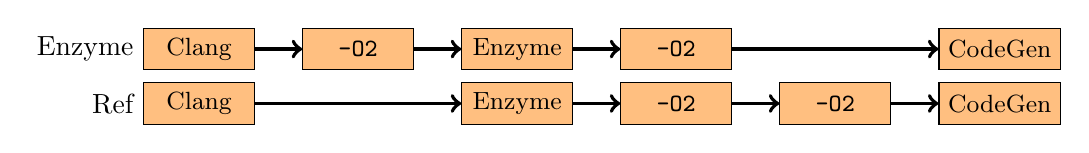
\begin{tikzpicture}[auto, node distance=.15cm and 0.6cm]

    \node [process, label=left:{Enzyme}] (clang1) {Clang};

    \node [process, right= of clang1] (opt1) {\texttt{-O2}};

    \node [process, right= of opt1] (enzyme1) {Enzyme};

    \node [process, right= of enzyme1] (popt1) {\texttt{-O2}};

    
    \node [process, label=left:{Ref}, below= of clang1] (clang2) {Clang};

    \node [process, below= of enzyme1] (enzyme2) {Enzyme};

    \node [process, right= of enzyme2] (opt2) {\texttt{-O2}};

    \node [process, right= of opt2] (popt2) {\texttt{-O2}};

    \node [process, right= of popt2] (cg2) {CodeGen};

    \node [process, above= of cg2] (cg1) {CodeGen};

    \draw [->, line width=0.5mm] (clang1) -- node {} (opt1);
    \draw [->, line width=0.5mm] (opt1) -- node {} (enzyme1);
    \draw [->, line width=0.5mm] (enzyme1) -- node {} (popt1);
    \draw [->, line width=0.5mm] (popt1) -- node {} (cg1);

    \draw [->, line width=0.5mm] (clang2) -- node {} (enzyme2);
    \draw [->, line width=0.5mm] (enzyme2) -- node {} (opt2);
    \draw [->, line width=0.5mm] (opt2) -- node {} (popt2);
    \draw [->, line width=0.5mm] (popt2) -- node {} (cg2);
  \end{tikzpicture}

\caption{The evaluation pipelines.}
  \label{fig:pipeline}
\end{figure}

We evaluate the Enzyme approach by measuring the runtime of seven benchmarks: the three reverse-mode benchmarks from Microsoft's machine-learning focused ADBench suite, and four additional tests that are technically interesting or represent potential use cases of Enzyme in practice. The ADBench suite includes bundle analysis (BA), a long short term memory model (LSTM), and a gaussian mixture model (GMM). We also differentiate two integrators (Euler, RK4) from the Odeint header-only ODE solver library ~\cite{ahnert2011odeint}; a simple Fast Fourier Fransform (FFT); and finite difference discretized simulation of the 2-dimensional Brusselator system (Bruss) ~\cite{feinberg1987chemical,yu2018mathematical}.

The two integrators are interesting for testing indirect function calls, complicated C++ headers, and foreign ODE solvers. The FFT test is interesting for demonstrating recursive functions. The Brusselator test demonstrates the utility in adjoint sensitivity analysis for ordinary differential equations, a widely applicable method with applications to PDE-constrained optimization~\cite{biegler2003large, li2004adjoint}, control theory~\cite{piasecki1997control}, and scientific machine learning like neural ODE's~\cite{rackauckas2020universal, chen2018neural}


\begin{figure}
    \centering

\begin{tabular}{cc}
\hspace*{-1cm}
\begin{minipage}[T]{0.69\linewidth}
\includegraphics[width=0.99\linewidth]{figs/all.pdf}
\end{minipage}
&
\begin{minipage}[T]{0.29\linewidth}
\hspace*{-1cm} {\scriptsize \begin{tabular}{r|c|c|c|c}
& Enzyme& Ref& Tapenade& Adept\\
BA& \textbf{0.250}& 0.442& 0.391& 1.447\\
LSTM& \textbf{2.405}& 4.426& 4.026& 7.540\\
GMM& 0.261& 0.482& \textbf{0.130}& 0.725\\
Euler& \textbf{0.185}& 14.258& N/A& 8.650\\
RK4& \textbf{3.929}& 12.904& N/A& 6.335\\
FFT& \textbf{0.182}& \textbf{0.182}& N/A& 2.439\\
Bruss& \textbf{0.182}& 0.183& 0.514& 3.444\\
\end{tabular}}
\end{minipage}
\end{tabular}
    \caption{\textbf{\textit{Left:}} Relative speedup of AD systems on the benchmark suite. A red X denotes programs that an AD system does not produce a correct gradient (after accounting for the Tapenade corrections present in ADBench). For each benchmark, we take the geometric mean of the runtime for all test cases, normalizing to the victor. A value of 1.0 denotes the fastest AD system tested for that benchmark, whereas a value of 0.5 denotes that an AD system produced a gradient which took twice as long. \textbf{\textit{Right:}} table with geometric mean runtime in seconds. N/A indicates a benchmark did not work with that system, perhaps producing incorrect results.}
    \label{fig:eval}
\end{figure}

To evaluate the effectiveness of AD on optimized IR, we construct two pipelines shown in Figure~\ref{fig:pipeline}. The Enzyme pipeline consists of running optimizations before Enzyme AD, followed by a second round of optimizations. The Reference (Ref) pipeline is identical to the Enzyme pipeline, except that AD is performed before the first round of optimization. This allows us to effectively evaluate the importance of optimization on AD without considering additional confounding factors (such as differing tape implementations) between Enzyme and existing source AD systems. We ran our experiments on a ``quiesced'' AWS c4.8xlarge instance with hyperthreading and Turbo Boost disabled. Taking the geometric mean across all benchmarks, Enzyme outperforms Reference by a factor of 2.851.

We also compare against the two fastest C/C++ AD tools evaluated in ADBench. These results are presented in Figure~\ref{fig:eval}. Enzyme demonstrate state-of-the-art performance for 7 of the 8 benchmarks. Furthermore the reference pipeline achieves similar performance to Tapenade on the BA and LSTM benchmarks, suggesting that Enzyme's advantage stems from running optimizations first. Tapenade's superior performance on GMM and Enzyme's superior performance on Bruss, however, can be explained by differences in how Enzyme and Tapenade implement their tape structures. Initial optimization also makes a significant impact on the Euler and RK4 tests, explaining much of the performance gap between Enzyme and Adept, whereas Enzyme's efficient tape structure explains its superior performance on FFT.


%We ran our experiments on a ``quiesced'' AWS c4.8xlarge instance with 60 GiB of memory and 18 cores. To minimize variance, we disabled hyperthreading and Turbo Boost.
\section{Conclusion}
\label{sec:conclusion}

 Future work: AD-specification opt
 GPU backend to generate GPU code from existing
 Take in in parallel/gpu from tapir/omp/etc
 Ham it up about don't make a new diffe programming unless you need
 cross language ad disc
 Future work: working with ML community to port phys engines/etc
\begin{ack}
Use unnumbered first level headings for the acknowledgments. All acknowledgments
go at the end of the paper before the list of references. Moreover, you are required to declare 
funding (financial activities supporting the submitted work) and competing interests (related financial activities outside the submitted work). 
More information about this disclosure can be found at: \url{https://neurips.cc/Conferences/2020/PaperInformation/FundingDisclosure}.


Do {\bf not} include this section in the anonymized submission, only in the final paper. You can use the \texttt{ack} environment provided in the style file to autmoatically hide this section in the anonymized submission.
\end{ack}

\bibliography{allpapers}

\end{document}